\documentclass[12pt, letterpaper, twoside]{article}
\usepackage[utf8]{inputenc}
\usepackage[margin=1in]{geometry}
\usepackage{graphicx}
\usepackage{float}
\usepackage{color}
\usepackage{hyperref}
\usepackage{listings}
\usepackage{spverbatim}
\usepackage{fancyvrb}
\usepackage{fvextra}
\title{}
\author{}
%
\makeatletter
\setlength{\@fptop}{0pt}
\makeatother
\usepackage[figurename=Fig.]{caption}
%
\begin{document}
\maketitle

\section{Bitcoin peer-to-peer protocol}\label{netintro}
\subsection{Connection and peer discovery}\label{peerdisc}
In order to establish a connection two peers need to exchange version messages over an unencrypted TCP channel in an handshake fashion as shown in \emph{Fig. 1}. The node that first sends a \texttt{version} message is said to be establishing an \emph{outgoing connection}. The receiving node sets up an \emph{ingoing connection} instead. Once the handshake is completed the connection is fully set up.

\begin{figure}[h]
	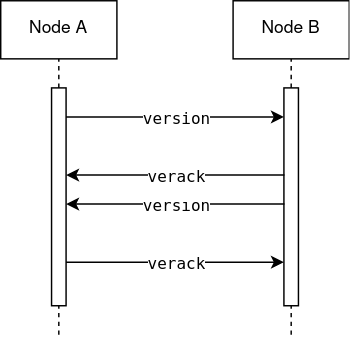
\includegraphics[width=.45\textwidth]{pict/BTCconnection.png}
	\centering
	\caption{Peers connection handshake}
\end{figure}

Each node is able to establish up to 8 outgoing connections and 117 ingoing connections, for a total of 125 connections. In order to keep its connections active, each peer sends a message to each neighbour at least once every thirty minutes. If more than ninety minutes pass without receiving anything from a neighbour, the connection is dropped. Each node always tries to keep eight outgoing connections active, therefore, upon dropping an outgoing connection, a node tries to connect to another address in its peer cache.

Nodes on fresh bootstrap make use of hardcoded \emph{DNS seeds} as their first mean to discover other peers. DNS seed servers are maintained by community members and provide clients with a list of addresses that can be either dynamically gathered through a periodic scan of the network or manually updated by server administrators. As a fallback option the user is able to specify through command line a list of addresses the client can connect to. Were both these two options to fail the client has a hardcoded list of peers it can directly connect to, though this is considered the last resort for bootstrapping peers.

Nodes at startup that were previously on the network shall first lookup peer names in their local address database, implemented as "peer.dat". The database contains the address of each peer the node has come to know during its lifetime in the network.

If the node has disconnected for a time too long, many of the addresses in the database may have become outdated or unreachable. A node that cannot connect to any address in the peer database or has spent up to eleven seconds trying to connect unsuccessfully to at least one of the peers in the database behaves as on fresh bootstrap and resolves to query a DNS first.

The use of a local address database, also called \emph{peer cache}, provides reconnecting peers a fully-decentralized way to join the network and is the first line of defence against \emph{fake bootstrap attacks}; the topic along with other security concerns is discussed in Chapter \ref{netsec}.

Peer discovery after the first connection of a node is carried on through the exchange of \texttt{addr} messages containing the address and port number of other peers in the network. On connection set up the two nodes exchange \texttt{addr} messages, as shown in \emph{Fig. 2}, providing each other with addresses from their local peer database.On top of that, every twenty-four hours each node advertises itself on the network with an \texttt{addr} message containing only its own address.

\begin{figure}[h]
	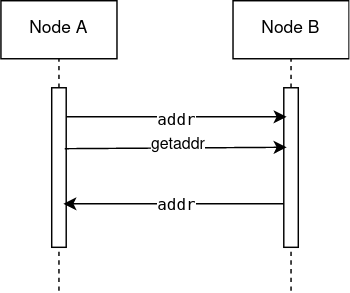
\includegraphics[width=.45\textwidth]{pict/BTCaddr.png}
	\centering
	\caption{Addresses exchange upon connection}
\end{figure}

 \texttt{addr} messages can contain at most one thousand addresses; additionally those containing ten or fewer addresses are relayed. This behaviour contributes to the gossiping of self-advertisement messages even though messages are relayed only to a small subset of neighbours, namely to a couple of peers.

\subsection{Peer database structure}\label{cachestruct}
The local peer database or cache serves the purpose of storing the addresses a node has come to know from \texttt{addr} messages and DNS seeds. The database is constituted of the \texttt{new} and the \texttt{tried} tables.

The \texttt{tried} table contains addresses of peers with whom the node has successfully established a connection in the past. It consists of 64 buckets that can store up to 64 unique addresses. Buckets are selected through a hash on the IP address.

The \texttt{new} table contains the addresses the node has not connected to and is therefore larger: it has 256 buckets of 64 addresses each.

Peer caches have been widely implemented in distributed systems so far as they are a fast and fully-decentralized way to rejoin the network after a disconnection. They allow peer-to-peer systems to overcome major issues at bootstrap time, mainly related to the presence of a single point of failure, i.e. bootstrap servers. Furthermore, they are the most scalable and efficient solution when compared to other decentralized mechanisms such as \textit{address probing}~\cite{decentrbootstrapp2p}.

\section{Bitcoin security concerns}\label{securityintro}
Bitcoin's decentralized, uncontrolled environment is open to a wide range of attacks, many of which can be applied to other cryptocurrencies as well. For this reason the following could be considered attack paradigms, with the same rationale, but different implementation amongst different cryptocurrency systems.

Attacks like \textit{double-spending} aim to exploit system deficiencies: a malicious user tries to spend, with different transactions, the same set of coins two times. Although proof-of-work consensus makes double-spending infeasible, the attack can be still executed through other approaches that manipulate peers, as with network partitions, or were other conditions to be met~\cite{doublespendfastpay}.

Double-spending can be also carried out were an attacker to hold the majority of the computing power, this condition is known as \textit{51\%} or \textit{majority} attack~\cite{51atk}. With the majority of the network's hash rate an attacker would also be able to fork the blockchain to its own advantage and prevent transactions and blocks from being verified; this represents the worst security threat for any cryptocurrency.

Blockchain forks can be exploited to engineer block races as in \textit{selfish mining} attacks, were the malicious user intentionally holds private his mined blocks~\cite{selfishmining},~\cite{leelavimolsilp2018selfish}. If the attacker successfully keeps his private chain longer than the public one it can release his mined blocks, thus claiming the rewards for himself and wasting other miners' computing power.

These are just a few attacks that can be driven onto Bitcoin, as this chapter serves only introductory purposes. In the following sections there is more on network attacks, which are the focus of this thesis. The interested reader can find complete security overviews in the works of Conti et al., Saad et al. and Wang et al.~\cite{completeattacksurvey},~\cite{saad2019attacksurface},~\cite{secpermissionlessblock}.

\subsection{Network security}\label{netsec}
Attacks that exploit vulnerabilities in the design and implementation of Bitcoin protocols and its peer-to-peer network fall under the category of network attacks.

Bitcoin is exposed to all the common threats that affect other peer-to-peer systems; these have been widely studied in the literature as in Touceda et al, 2012~\cite{toucedafakeboot}. The aim of this section is to understand how these attacks apply to Bitcoin and what are its defences.

The attacks reviewed in this chapter mainly focus on topology manipulation, with the exception of the \emph{DDoS} attack.

Often the goal of the attacker is to alter the view of the network of a node, or group of nodes, by sending false network information with the purpose of monopolizing its connections.

Thus victims become isolated and a network partition is created. This condition, often referred to as the \textit{eclipsing} of node, is inherently dangerous for the attacker can alter the node's view of the blockchain, waste its computing power or simply cut off its communications.

More specifically, eclipsed victims are vulnerable to \textit{N-confirmation double spending} and selfish mining attacks; furthermore 51\% attacks are easier to launch~\cite{eclipseatk}. For these reasons network attacks on topology are fundamental enablers for mining and spending attacks~\cite{dotan2020surveychallenges}.\\

In the following sections the reader can find both the attacks performed during the simulations reported in this thesis along with other network level attacks. These were added to better understand the mechanisms exploitable to carry out network attacks on cryptocurrencies.

\subsubsection{Fake bootstrapping attack}\label{fakeboot}
Every peer-to-peer system needs some mean to let nodes join the network: in Bitcoin bootstrapping nodes need to rely on the information provided by some other peer in the network.

In a fake bootstrapping attack the peers contacted while a node is still initiating its connections, and hence its knowledge of the network, flood the bootstrapping peer with malicious addresses.

The results in Chapter~\ref{res} show how feeding bogus information to a joining node can seriously influence its view of the network and lead to network partitions and peer eclipsing. This condition would also increase the efficacy of other network-level attacks, such as a DDoS, and the success rate of spending and mining attacks~\cite{eclipseatk}.\\

Prevention is done by ensuring a node can contact a trustworthy peer when joining the network. Peer caches and centralized bootstrap services serve this purpose, allowing joining nodes to make use of old neighbours while having central bootstrap servers as a fallback.

Other solutions have been implemented and tested over time, though their drawbacks usually exceed the benefits. As an example, randomly probing the address space, scouting for peers, decentralizes the bootstrap process and increases the variance of the network knowledge, but may not work if peers are behind NATs or firewalls and increases the latency for joining the network~\cite{decentrbootstrapp2p}~\cite{localityaware}. In 2012,  Touceda et al. discuss fake bootstrapping along with other security threats in their survey~\cite{toucedafakeboot}.

Bitcoin employs many countermeasures, and overcomes other bootstrap issues, with its peer cache implementation mixed with external mechanisms: each node contacts its stored addresses for successive connections and aims to establish multiple outgoing connections, thus it does not rely on a single bootstrap node. On top of that, DNS seeds provide a reliable external bootstrap service and the user is given the ability to manually insert addresses to connect to~\cite{mahmoud_netsec_boot}.

\subsubsection{Eclipse attack}\label{eclipse}
During an eclipse attack the victim is flooded with a multitude of incoming connections from an attacker and fed bogus network information, i.e. peer addresses, that will fill up the peer cache. 

Upon restarting, with high probability the victim will form all of its eight outgoing connections with malicious IP addresses, thus finding itself eclipsed. As described in Section~\ref{netsec} this greatly enhances the efficacy and impact of other attacks.

In 2015, Heilman et al. widely describe eclipse attacks and suggest many countermeasures to harden the network, a few of which were implemented in Bitcoin Core~\cite{eclipseatk}. As part of the adoption of these countermeasures, the number of buckets in \texttt{new} and \texttt{tried} has been increased, the addresses have become deterministically hashed to a single slot inside a bucket and the heavy bias towards addresses with fresher timestamps when choosing new connections has been removed.

\subsubsection{Sybil attack}\label{sybil}

\subsubsection{DDoS attack}\label{ddos}
Distributed Denial of Service (DDoS).

\section{Results}\label{res}
attack description
methods adopted, metrics and software
results obtained: show them, then discuss them


















\bibliographystyle{plain}
\bibliography{bib.bib}

\end{document}